\documentclass[sigconf,authordraft]{acmart}

%%
%% \BibTeX command to typeset BibTeX logo in the docs
\AtBeginDocument{%
  \providecommand\BibTeX{{%
    \normalfont B\kern-0.5em{\scshape i\kern-0.25em b}\kern-0.8em\TeX}}}

%% Rights management information.  This information is sent to you
%% when you complete the rights form.  These commands have SAMPLE
%% values in them; it is your responsibility as an author to replace
%% the commands and values with those provided to you when you
%% complete the rights form.
\setcopyright{acmcopyright}
\copyrightyear{2020}
\acmYear{2020}
%\acmDOI{10.1145/1122445.1122456}

%% These commands are for a PROCEEDINGS abstract or paper.
\acmConference[PEARC '20]{PEARC '20}{July 26-30, 2020}{Portland, OR }
%\acmBooktitle{Woodstock '18: ACM Symposium on Neural Gaze Detection,
%  June 03--05, 2018, Woodstock, NY}
%\acmPrice{15.00}
%\acmISBN{978-1-4503-XXXX-X/18/06}


%%
%% Submission ID.
%% Use this when submitting an article to a sponsored event. You'll
%% receive a unique submission ID from the organizers
%% of the event, and this ID should be used as the parameter to this command.
%%\acmSubmissionID{123-A56-BU3}

%%
%% The majority of ACM publications use numbered citations and
%% references.  The command \citestyle{authoryear} switches to the
%% "author year" style.
%%
%% If you are preparing content for an event
%% sponsored by ACM SIGGRAPH, you must use the "author year" style of
%% citations and references.
%% Uncommenting
%% the next command will enable that style.
%%\citestyle{acmauthoryear}

%%
%% end of the preamble, start of the body of the document source.
\begin{document}

%%
%% The "title" command has an optional parameter,
%% allowing the author to define a "short title" to be used in page headers.
\title{Benchmark informed software upgrades at Quest, Northwestern's HPC cluster}

%%
%% The "author" command and its associated commands are used to define
%% the authors and their affiliations.
%% Of note is the shared affiliation of the first two authors, and the
%% "authornote" and "authornotemark" commands
%% used to denote shared contribution to the research.
\author{Sajid Ali}
\orcid{0000-0003-2186-4636}
\affiliation{%
  \institution{Applied Physics, Northwestern University}
  \streetaddress{2145 Sheridan Road}
  \city{Evanston}
  \state{Illinois}
  \postcode{60208}
}
\email{sajidsyed2021@u.northwestern.edu}

\author{Alex Mamach}
\affiliation{%
	\institution{NUIT, Northwestern University}
	\streetaddress{2145 Sheridan Road}
	\city{Evanston}
	\state{Illinois}
	\postcode{60208}
}
\email{alex.mamach@northwestern.edu}


\author{Alper Kinaci}
\affiliation{%
\institution{NUIT, Northwestern University}
  \streetaddress{2145 Sheridan Road}
  \city{Evanston}
  \state{Illinois}
  \postcode{60208}
  }
\email{akinaci@northwestern.edu}

%%
%% By default, the full list of authors will be used in the page
%% headers. Often, this list is too long, and will overlap
%% other information printed in the page headers. This command allows
%% the author to define a more concise list
%% of authors' names for this purpose.
%%\renewcommand{\shortauthors}{Trovato and Tobin, et al.}

%%
%% The abstract is a short summary of the work to be presented in the
%% article.
\begin{abstract}
  We present the work performed at Quest, a high performance computing cluster at Northwestern University regarding benchmarking of software performed to guide software upgrades. We performed extensive evaluation of all MPI modules present on the system for functionality and performance in addition to testing a strategy to deploy architecture optimized software that can be loaded dynamically at runtime.
\end{abstract}

%%
%% The code below is generated by the tool at http://dl.acm.org/ccs.cfm.
%% Please copy and paste the code instead of the example below.
%%
\begin{CCSXML}
	<ccs2012>
	<concept>
	<concept_id>10011007.10011006.10011071</concept_id>
	<concept_desc>Software and its engineering~Software configuration management and version control systems</concept_desc>
	<concept_significance>500</concept_significance>
	</concept>
	<concept>
	<concept_id>10011007.10011006.10011073</concept_id>
	<concept_desc>Software and its engineering~Software maintenance tools</concept_desc>
	<concept_significance>300</concept_significance>
	</concept>
	</ccs2012>
\end{CCSXML}

\ccsdesc[500]{Software and its engineering~Software configuration management and version control systems}
\ccsdesc[300]{Software and its engineering~Software maintenance tools}

%%
%% Keywords. The author(s) should pick words that accurately describe
%% the work being presented. Separate the keywords with commas.
\keywords{software management, 	software builds, software automation}

%%
%% This command processes the author and affiliation and title
%% information and builds the first part of the formatted document.
\maketitle

\section{Introduction}

Quest is a heterogeneous HPC cluster\cite{quest} at Northwestern University consisting of Intel Haswell/Broadwell/Skylake/Cascale Lake nodes with varying interconnects which recently transitioned to SLURM\cite{slurm} as the resource manager and the job scheduler. The cluster operates with very high uptimes and generally shuts down for a week once every academic year for maintenance. While this high uptime is great for research throughput, it compresses critical maintenance tasks into that week and makes the operators prioritize in place upgrades over major redesigns. While such an operations scheme works in the short run, managing a large set of software stacks that were installed at various points in time becomes challenging since the software stack was kept stable even through downtime cycles that involved major and minor OS upgrades.

This has led to a bloated software stack and sometimes inconsistencies in naming schemes for modules and executables. This is challenging to continuously benchmark for functionality and performance. Thus, we are motivated to develop a strategy to maintain our software stacks that will enable us to provide functional and efficient software for our users while reducing the maintenance and support workload for the operators and software specialists. In addition to the above, we also face an immediate need to make MPI launchers compatible with srun as a SLRUM update is on the agenda for the next downtime.

In this article, we present our ongoing project to modernize MPI installations and the results of benchmarking studies that inform our plans for deprecating modules. We also discuss the preliminary tests on our beta cluster for a strategy to deploy optimized builds for each architecture that are dynamically loaded at runtime based upon the nodelist for the job.

\section{MPI upgrade project milestones}
The authors
- Deployment of a beta cluster with SLURM 19 (later updated to SLURM 20)
- Benchmark existing and recompiled MPI on the beta cluster
- Deployment of updated performance libraries (UCX, PMIx) on the production cluster
- User communication informing the module deprecation
- User tests using recompiled or new MPI applications on beta cluster 
- MPI modules transition along with SLURM update on production cluster

During the submission of this manuscript  

 

The MPI upgrade project involves 


\section{MPI libraries}
Over the 10-year life of Quest cluster, multiple versions of libraries proving functionality specified by the message passing interface standard \cite{mpi_3_1,mpi_2_2} were installed. Some of these are quite old (before major OS version upgrades) and the naming scheme for the corresponding module files is inconsistent. To test these libraries for functionality and performance, we compiled and executed two point-to-point benchmarks, bandwidth and latency from the OSU micro-benchmarks suite \cite{osu_bench_website}. Since none of MPI modules were installed with SLURM support, we wrote a bash script to automate the tests. The results are presented in the figure \ref{fig:currmpi}.

\begin{figure}[h]
	\centering
	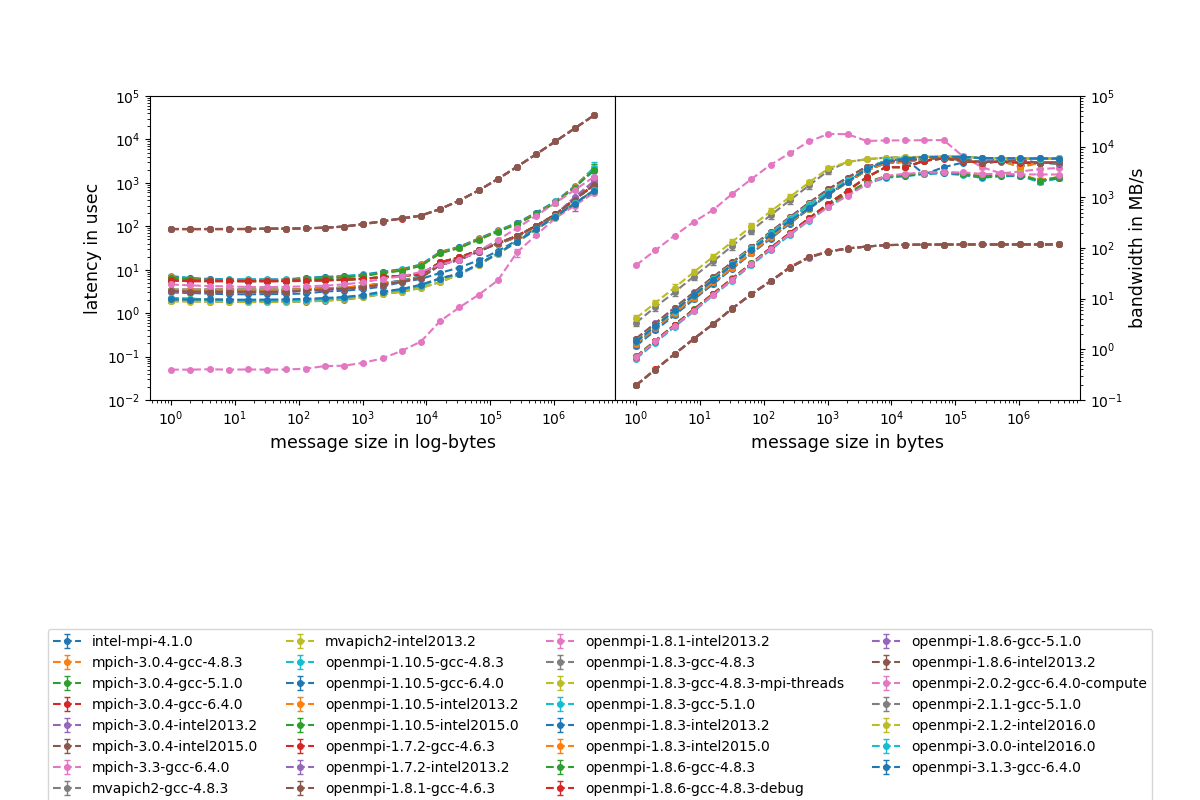
\includegraphics[width=\linewidth]{curr_mpi_combined}
	\caption{Benchmark of currently available MPI builds}
	\Description{Benchmark of currently available MPI builds}	  \label{fig:currmpi}
\end{figure}

In total, $42\%$ of the available MPI libraries were faulty with $28\%$ being nonfunctional (failure to compile or run) and the rest being less then optimal efficiency.

\subsection{Improvements}
 
Spack\cite{spack} was used to build new versions of MPI libraries with SLURM support. This allows us to automate a large set of parameterized builds and eases the testing. Alongside testing the new installations for srun launcher support, we also tested the relative performance of the UCX transport layer \cite{shamis2015ucx,openucx-website}. Unified Communication X (abbreviated as UCX) is a portable, high performance middleware that sits between programming models (like MPI, PGAS, charm++, etc) and network device drivers. The results of benchmarks with new installations are presented in the figure \ref{fig:currmpi}. 

\begin{figure}[h]
	\centering
	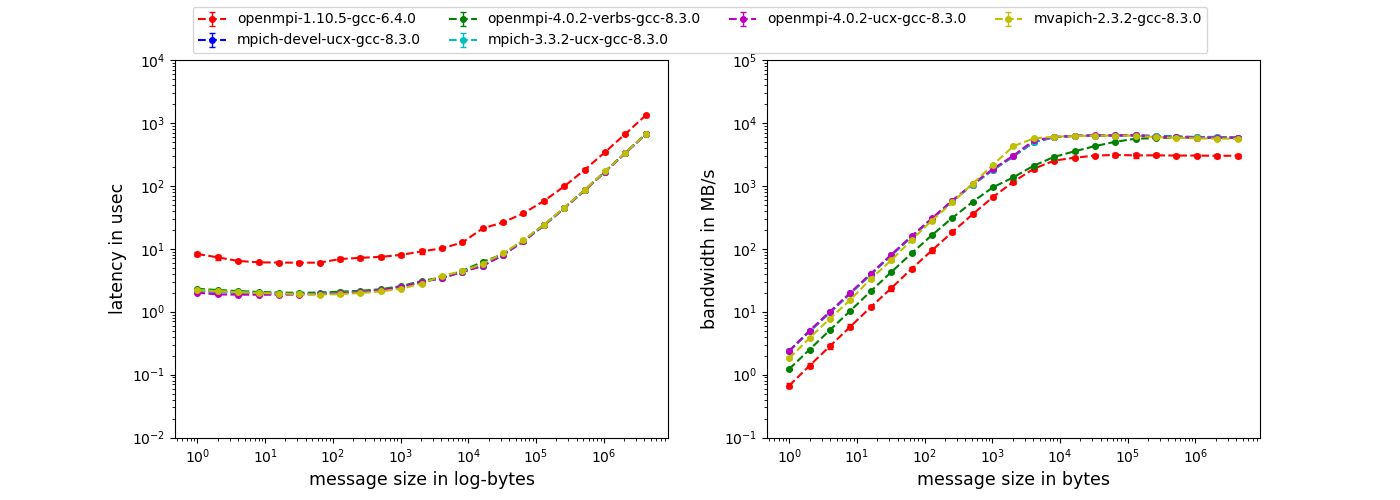
\includegraphics[width=\linewidth]{new_mpi}
	\caption{Benchmark of new MPI builds}
	\Description{Benchmark of new MPI builds}
	\label{fig:newmpi}
\end{figure}

As indicated in a recent OpenMPI deployment guide \cite{openmpi_deployment_tuning}, newer versions of the libraries configured with UCX transport layer perform better. We have thus  decided to use the UCX transport layer for all MPI libraries. In addition to this, we also plan to enable the PMIx plugin \cite{slurm_pmix_sc17,slurm_pmix_2019} in slurm to use the PMIx process management standard \cite{pmix,pmix_website} (implemented via the OpenPMIx library \cite{openpmix_website}) which improves the job startup time. We also note that the slurm plugin for PMIx allows it optionally use UCX for communication via a slurm plugin for UCX.

\subsection{Deploying UCX and PMIx}
While UCX was installed on the GPFS filesystem for convenience of testing, we plan to install it on the node-local filesystem (specifically at $/usr/local$) of each compute node given it's nature as a widely used runtime dependency for MPI libraries. We already had an older version of UCX, $1.4.0$ available (as part of the Mellanox driver installations) and used this alongside an installation of OpenPMIx \cite{openpmix_website}, version $2.2.3$ for testing. Unfortunately due to a bug in the slurm plugin \cite{slurm_ucx_bug}, this configuration led to crash during the job start which reuqires ucx to be installed with rdma-core \cite{rdmacore_repository}(which provide the user space components for the IB drivers) dependency or update the drivers to a newer version.

Since there are no plans on updating the infibinand dirvers, we first attempted at manually creating binaries (in the $.rpm$ format using $rpm-builder$ tool) for UCX and PMIx that overcome the aforementioned bug. We had no success with this approach as we were unable to properly patch the libraries.

Thus, we plan to use spack \cite{spack} to install the libraries to a common prefix (by using a filesystem view in an environment) and create an rpm binary from this for easy deployment on the compute nodes.

\section{Node arch dependent software}

Given the challenges in maintaining a complex software stack that includes a multitude of combinations between applications, versions, compilers and dependencies, achieving optimal software performance (as available via generating optimized binaries for each architecture) was not prioritized. While this was not a major concern in the past, the increase in the CPU-architecture heterogeneity in the recent years, such a deployment strategy severely degrades productivity of the cluster. Thankfully, due to recent developments in the spack package manager, we are able to build multiple versions of each library, each optimized for a different architecture for optimal productivity of the cluster. 

\subsection{Benchmarks}
We benchmarked optimzed builds for two of our most commonly used applications, LAMMPS\cite{lammps} and Gromacs\cite{gromacs_1995,gromacs_2015} against the currently available installations on the oldest processor generation, "Haswell". We chose the Lennard-Jones liquid benchmark for LAMMPS available as part of the official benchmark suite \cite{lammps_bench} and a benchmark from the Unified European Applications Benchmark Suite \cite{ueabs_prace,ueabs_repo} for GROMACS. The results of these tests are presented in the Table \ref{tab:bench_apps} which shows that there are substantial benefits to deploying node architecture specific software even on our oldest nodes.

\begin{table}
	\caption{Optimized builds on Haswell nodes}
	\label{tab:bench_apps}
	\begin{tabular}{ccl}
		\toprule
		Software &Current&Optimized\\
		\midrule
		LAMMPS & 765.8 timesteps/day&1013.4 timesteps/day\\
		GROMACS & 1.78 ns/day&2.00 ns/day\\
		\bottomrule
	\end{tabular}
\end{table}

\subsection{Deployment Strategy}
On Quest, users are not required to choose a partition and the jobs are assigned to nodes dynamically based on availability. Thus, we are faced with the following deployment challenge : how do we deploy optimized builds for each processor family but not require our users to choose the exact build of the application for their job ?

To answer the above, we have chosen a simple strategy where we configure a task prolog script for SLURM that automatically sets the modulepath based on $SLURM\_NODELIST$. We tested this on a virtual SLURM cluster with two noes on a laptop provisioned by four docker containers tied together via docker-compose using an existing repository \cite{slurmdocker_repository} for the same developed by SciDAS (Scientific Data Analysis At Scale).

\begin{verbatim}
short_list=${SLURM_JOB_NODELIST##worker}
if [ $short_list == "01" ]
then
echo "export MODULEPATH=/home/path1"
fi
if [ $short_list == "02" ]
then
echo "export MODULEPATH=/home/path2"
fi
\end{verbatim}

\section{Conclusion}

Thus, we have effectively used benchmarking tests that gives us valuable insight regarding the health of the software on the Northwestern-Quest high performance compute cluster. This work will inform our plans to deprecate and eventually remove non-functional and non-performant software. Moreover, executing the node-optimized software strategy in the future would enable a significant enhancement in the productivity of the cluster.

%%
%% The acknowledgments section is defined using the "acks" environment
%% (and NOT an unnumbered section). This ensures the proper
%% identification of the section in the article metadata, and the
%% consistent spelling of the heading.
\begin{acks}
To various mailing lists, slack channels and forums including but not limited to mpich-discuss, slurm-info, spack-users.
\end{acks}

%%
%% The next two lines define the bibliography style to be used, and
%% the bibliography file.
\bibliographystyle{ACM-Reference-Format}
\bibliography{pearc20}

%%
%% If your work has an appendix, this is the place to put it.
%\appendix
%\section{Research Methods}
%\subsection{Part One}
%Lorem ipsum dolor sit amet, consectetur adipiscing elit. Morbi
%\subsection{Part Two}
%Etiam commodo feugiat nisl pulvinar pellentesque. Etiam auctor sodales
%\section{Online Resources}
%Nam id fermentum dui. Suspendisse sagittis tortor a nulla mollis, in

\end{document}
\endinput
%%
%% End of file `sample-authordraft.tex'.
